% TAREA 1 PROGRA 2






% PROBLEMA 1.1
\begin{mdframed}[style = warning]
	\begin{problem}
		($1.1$) Respondiendo las preguntas para los autómatas dados:
			\begin{enumerate}[a)]
				\item El estado inicial de $M_1$ es $q_o = q_1$, y de $M_2$ es $q_o = q_1$.
				\item Los estados aceptados de $M_1$ es $F = \{ q_2 \}$ y de $M_2$ es $F = \{ q_1,q_4 \}$.
				\item La secuencia en $M_1$ es $q_1,q_2,q_3q_1,q_1$. Para $M_2$ es $q_1,q_1,q_1,q_2,q_4$.
				\item De dicha palabra, solo el automata $M_2$ lo acepta.
				\item La cadena vacía no es aceptada.
			\end{enumerate}
	\end{problem}
\end{mdframed}











% PROBLEMA 2.1
\begin{mdframed}[style = warning]
	\begin{problem}
		($1.3$) Para el automata dado, el diagrama de estado es:
		\begin{figure}[H]
			\centering
			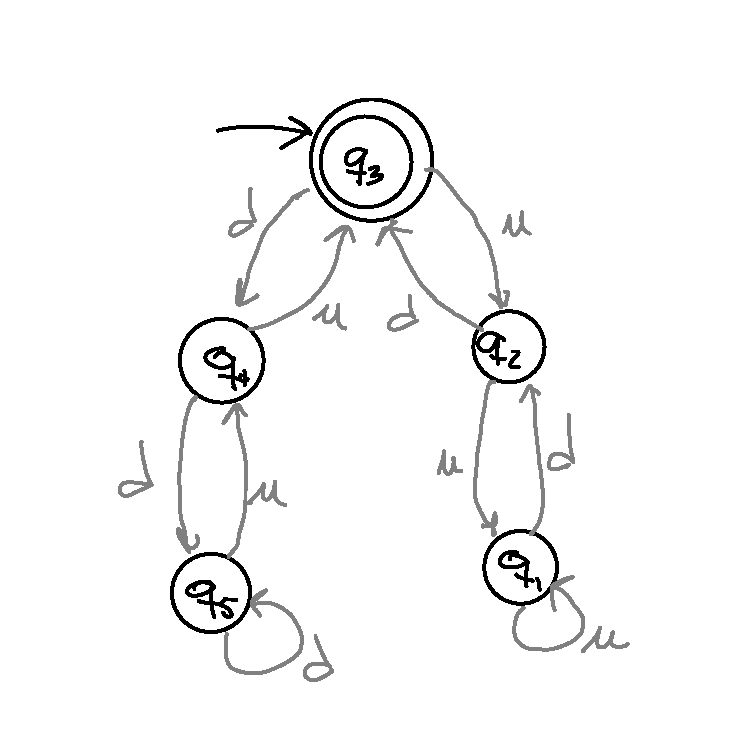
\includegraphics[scale=0.7]{Images/1-3.pdf}
			\caption{Diagrama de Estado, creado en \textit{Xournal}}
			\label{1-3}
		\end{figure}		 
	\end{problem}
\end{mdframed}












\begin{mdframed}[style = warning]
	\begin{problem}
		($1.4$) 	 
	\end{problem}
\end{mdframed}










\begin{mdframed}[style = warning]
	\begin{problem}
		($1.6$) 	 
	\end{problem}
\end{mdframed}









\begin{mdframed}[style = warning]
	\begin{problem}
		($1.8$) 	 
	\end{problem}
\end{mdframed}














\begin{mdframed}[style = warning]
	\begin{problem}
		($1.11$) 	 
	\end{problem}
\end{mdframed}
















\begin{mdframed}[style = warning]
	\begin{problem}
		($1.12$) 	 
	\end{problem}
\end{mdframed}














\begin{mdframed}[style = warning]
	\begin{problem}
		($1.14$) 	 
	\end{problem}
\end{mdframed}











\begin{mdframed}[style = warning]
	\begin{problem}
		($1.16$) 	 
	\end{problem}
\end{mdframed}












\begin{mdframed}[style = warning]
	\begin{problem}
		($1.17$) 	 
	\end{problem}
\end{mdframed}










\begin{mdframed}[style = warning]
	\begin{problem}
		($1.19$) 	 
	\end{problem}
\end{mdframed}












\begin{mdframed}[style = warning]
	\begin{problem}
		($1.21$) 	 
	\end{problem}
\end{mdframed}




















